\section{路线构建}
\label{sec:route}

\subsection{显著性场与稀疏增广树}

设归一化原始RGB图像为 $I\in[0,1]^{H\times W\times3}$。确定性算法生成显著性场 $S\in[0,1]^{H_r\times W_r}$。默认使用频率调谐Lab对比度 \cite{achanta2009frequency}，随后进行高斯平滑。模型从 $I$ 读取RGB；$S$ 只负责构建路线并提供路线属性。

在路线网格外增加一圈低于场值范围的边框，使接触图像边缘的轮廓闭合。每个网格单元固定按西北到东南的对角线剖分，相同标量值使用确定性的符号微扰。保留扫描层级之前，先在完整分片线性场上建立等高线树 $T$。补边后的矩形单连通，因此 $T$ 无环。树可以同时包含分裂和汇合鞍点，但同一次分裂产生的兄弟支路不会再次汇合；汇合只组合具有独立低值来源的分支。有孔洞的定义域需要改用Reeb图。

在 $L$ 个常规层级提取闭合轮廓，删除低于周长和面积阈值的小圈，并把其余轮廓插入对应树弧。没有保留轮廓的路径被收缩，得到稀疏执行树 $T_A$。这样，树负责跨层拓扑，细小分支不必消耗Token；法线碰到哪个对象都不会改变树边。

热力图平滑后，在路线网格上只计算一次 $3\times3$ Sobel场 $G=(G_x,G_y)$。所有轮廓共享这张场。

\subsection{统一的Sobel方向、密度与锚点}

对周长为 $P_C$ 的保留轮廓 $C$，先确定唯一点数：
\begin{equation}
N_C=\max\!\left(N_{\min},\operatorname{round}(P_C/\delta_0)\right).
\label{eq:budget-zh}
\end{equation}
默认 $N_{\min}=16,\delta_0=2$。点数没有语义上的最大值；长圈进入更大的长度桶，或者使用不丢点的精确分块扫描。变密度操作只能移动固定数量的点，不能让某个局部额外产生Token。

先把轮廓统一定向为顺时针，再沿弧长均匀放置 $M_C=2N_C$ 个试探点。设试探点为 $u_i$，按照统一环绕方向确定的单位法线为 $n_i$。在Sobel场中双线性读取后，得到一个带符号的法线响应：
\begin{equation}
r_i=G(u_i)^{\top}n_i.
\label{eq:sobel-response-zh}
\end{equation}
它的符号表示哪一侧热力值升高。若所有 $r_i$ 的平均值不小于零，说明正法线整体指向高值侧，整圈普通法线统一选择负法线侧；否则统一选择正法线侧。平均值恰为零时固定选择负法线侧。每个圈只作一次方向判断，不允许采样点各自改变左右方向。

绝对强度 $g_i=|r_i|$ 表示热力图跨越轮廓时变化得多快。沿闭环用 $(1,2,3,2,1)/9$ 平滑一次，得到 $\bar g_i$。令 $m_C$ 为正值 $\bar g_i$ 的中位数；如果整圈没有正响应，则全部密度权重设为1。否则：
\begin{equation}
w_i=\operatorname{clip}\!\left(\frac{\bar g_i}{m_C+\epsilon},1,3\right).
\label{eq:density-zh}
\end{equation}
弱变化区域保持基础密度，强变化区域获得更多点，最大权重限制避免小区域耗尽点数预算。当标量层级间隔固定时，较大的法线方向梯度也近似表示相邻等高线距离更短。

在尚未截断的平滑强度 $\bar g_i$ 中选择最大值所在试探点作为锚点 $p_0$；并列时选择图像坐标 $(y,x)$ 字典序最小的点。因此，同一批Sobel测量同时确定读取侧、采样密度和起止点，试探阶段不需要碰撞查询。

对每个试探区间，把实际弧长乘以两端平均权重，得到加权弧长。以 $p_0$ 为起点，在累计加权弧长上等间隔放置恰好 $N_C$ 个最终点，并强制保留 $p_0$。高权重区间的点更近，但总点数不变。整个过程不拉伸、不截断，也不补造几何点。顺、逆时针扫描使用同一组物理点的相反顺序。

只有重采样结束后才进行射线碰撞查询。每个最终点向整圈选定的普通侧发射射线，直到首次正向碰到其他保留轮廓折线或补边框；忽略起点接触和本轮廓的两条相邻线段。终止圈还会向相反侧发射第二条射线。路线坐标映射回原图后，RGB与显著性都用双线性插值读取。试探点本身不成为模型Token。

\begin{figure*}[t]
    \centering
    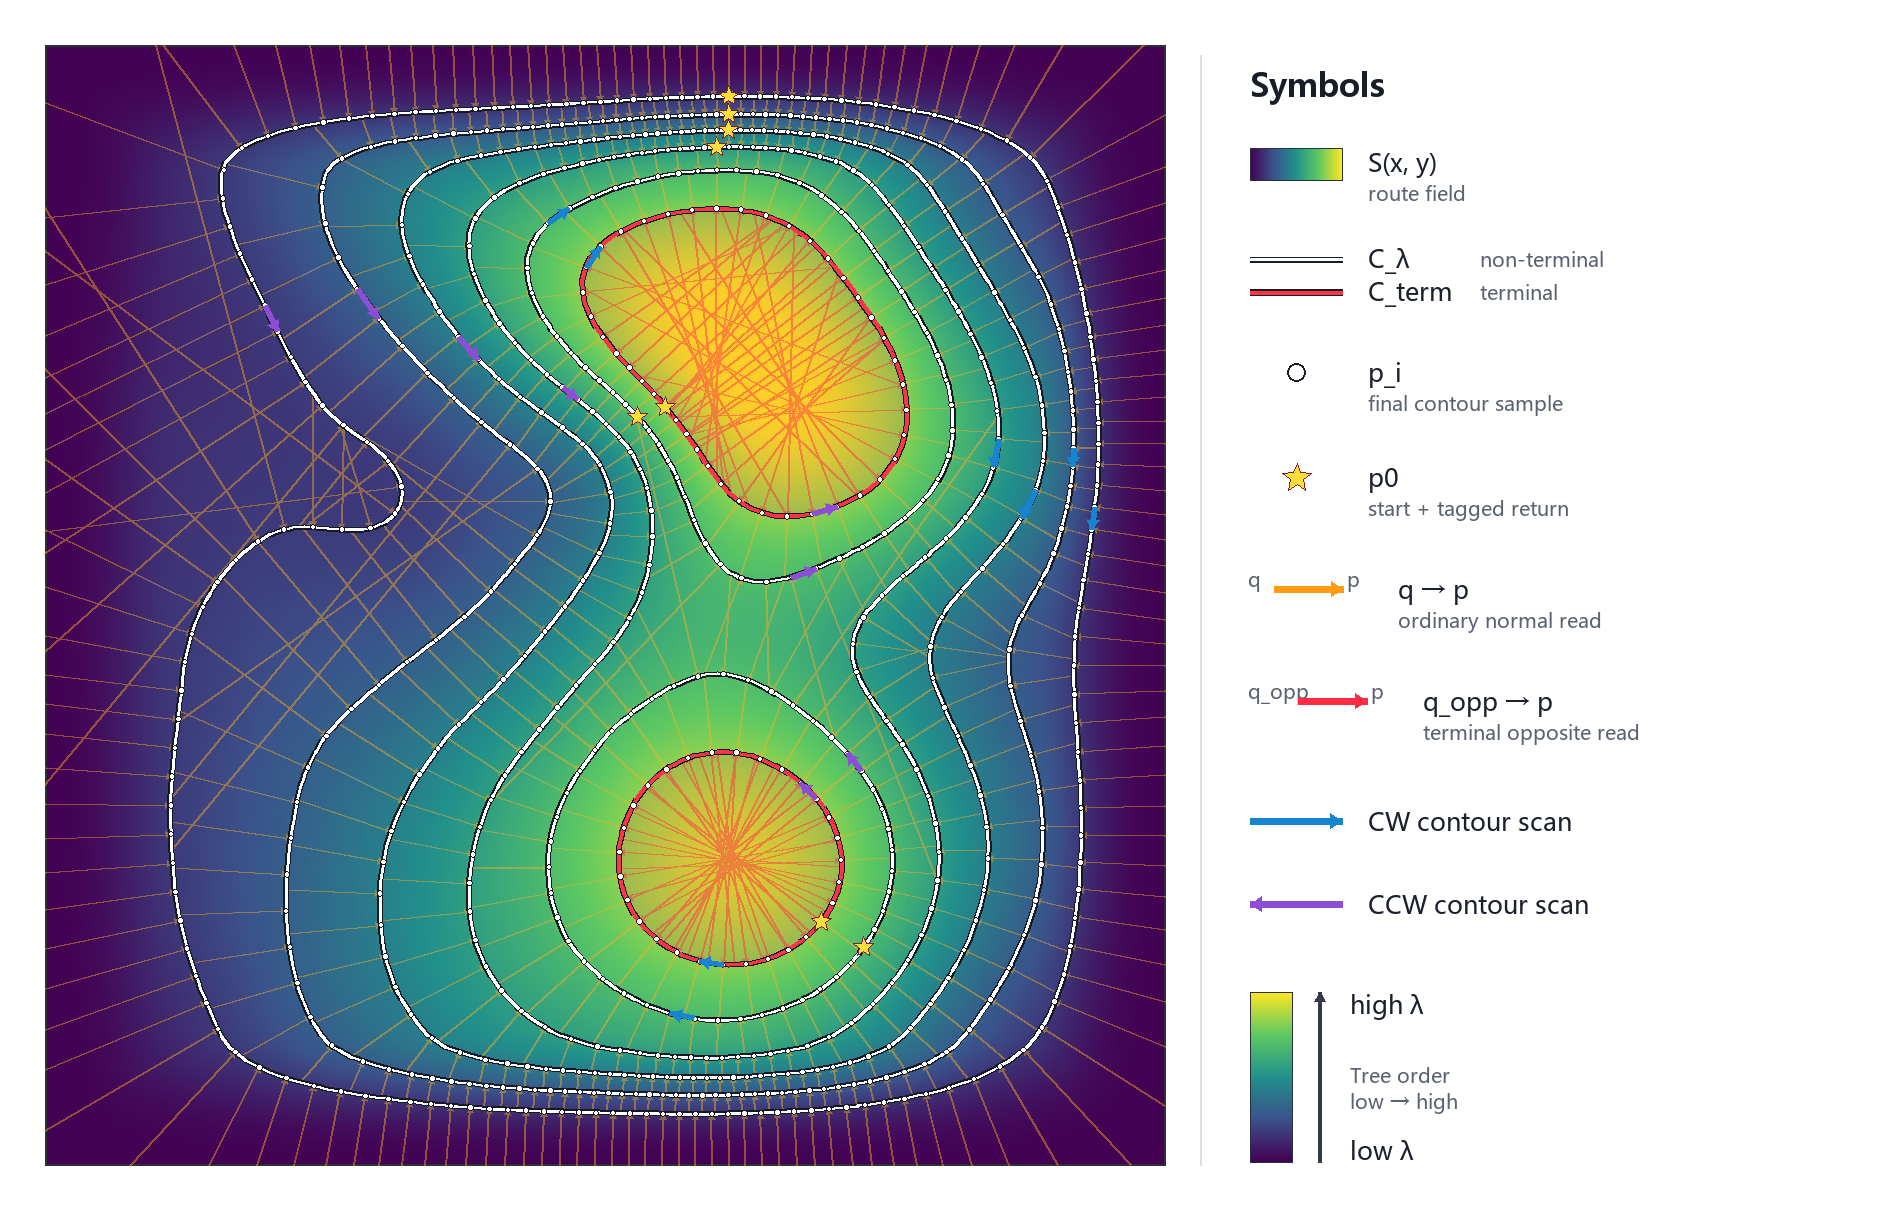
\includegraphics[width=0.84\textwidth]{figures/topocontour_paper_figure.png}
    \caption{按照本文规则生成的一条实际路线。白线表示保留的非终止轮廓；红线及浅红区域表示每条可见树枝最后保留的终止圈。橙色箭头表示Normal Mamba从首次碰撞点 $q$ 读回轮廓点 $p$ 的普通侧法线；红色箭头表示仅在终止圈补读的相反侧法线。星号表示共同起点和带Tag返回点 $p_0$，蓝色与紫色箭头表示两个闭环方向。}
    \label{fig:local}
    \vspace{0.35em}
    \begin{minipage}{0.84\textwidth}
    \small\textbf{设计哲学。}
    这条路线并不把低显著性区域判定为无用信息，也不删除它们。宽泛背景先进入历史；Sobel变化较弱的地方采样相对稀疏，而轮廓变化明显、位于树枝终点的证据后进入并更靠近带Tag的读出。因此，选择性遗忘在这里被用作一种注意力调度：较弱背景可以逐渐变模糊但仍然存在，辨识度较高的证据则较少受到后续更新影响。这只是归纳偏置，并不保证Mamba无损记忆。由于几何路线在扫描前已经确定，而且各轮廓的局部编码互相独立，图像相关的顺序仍可保持法线之间和轮廓之间的并行执行。
    \end{minipage}
\end{figure*}
